\documentclass[tikz,border=0pt]{standalone}
\usepackage{lmodern}
\usetikzlibrary{arrows.meta}
\definecolor{badge}{HTML}{D62728}
\definecolor{signal}{HTML}{000000}
\definecolor{accent}{HTML}{000000}
\begin{document}
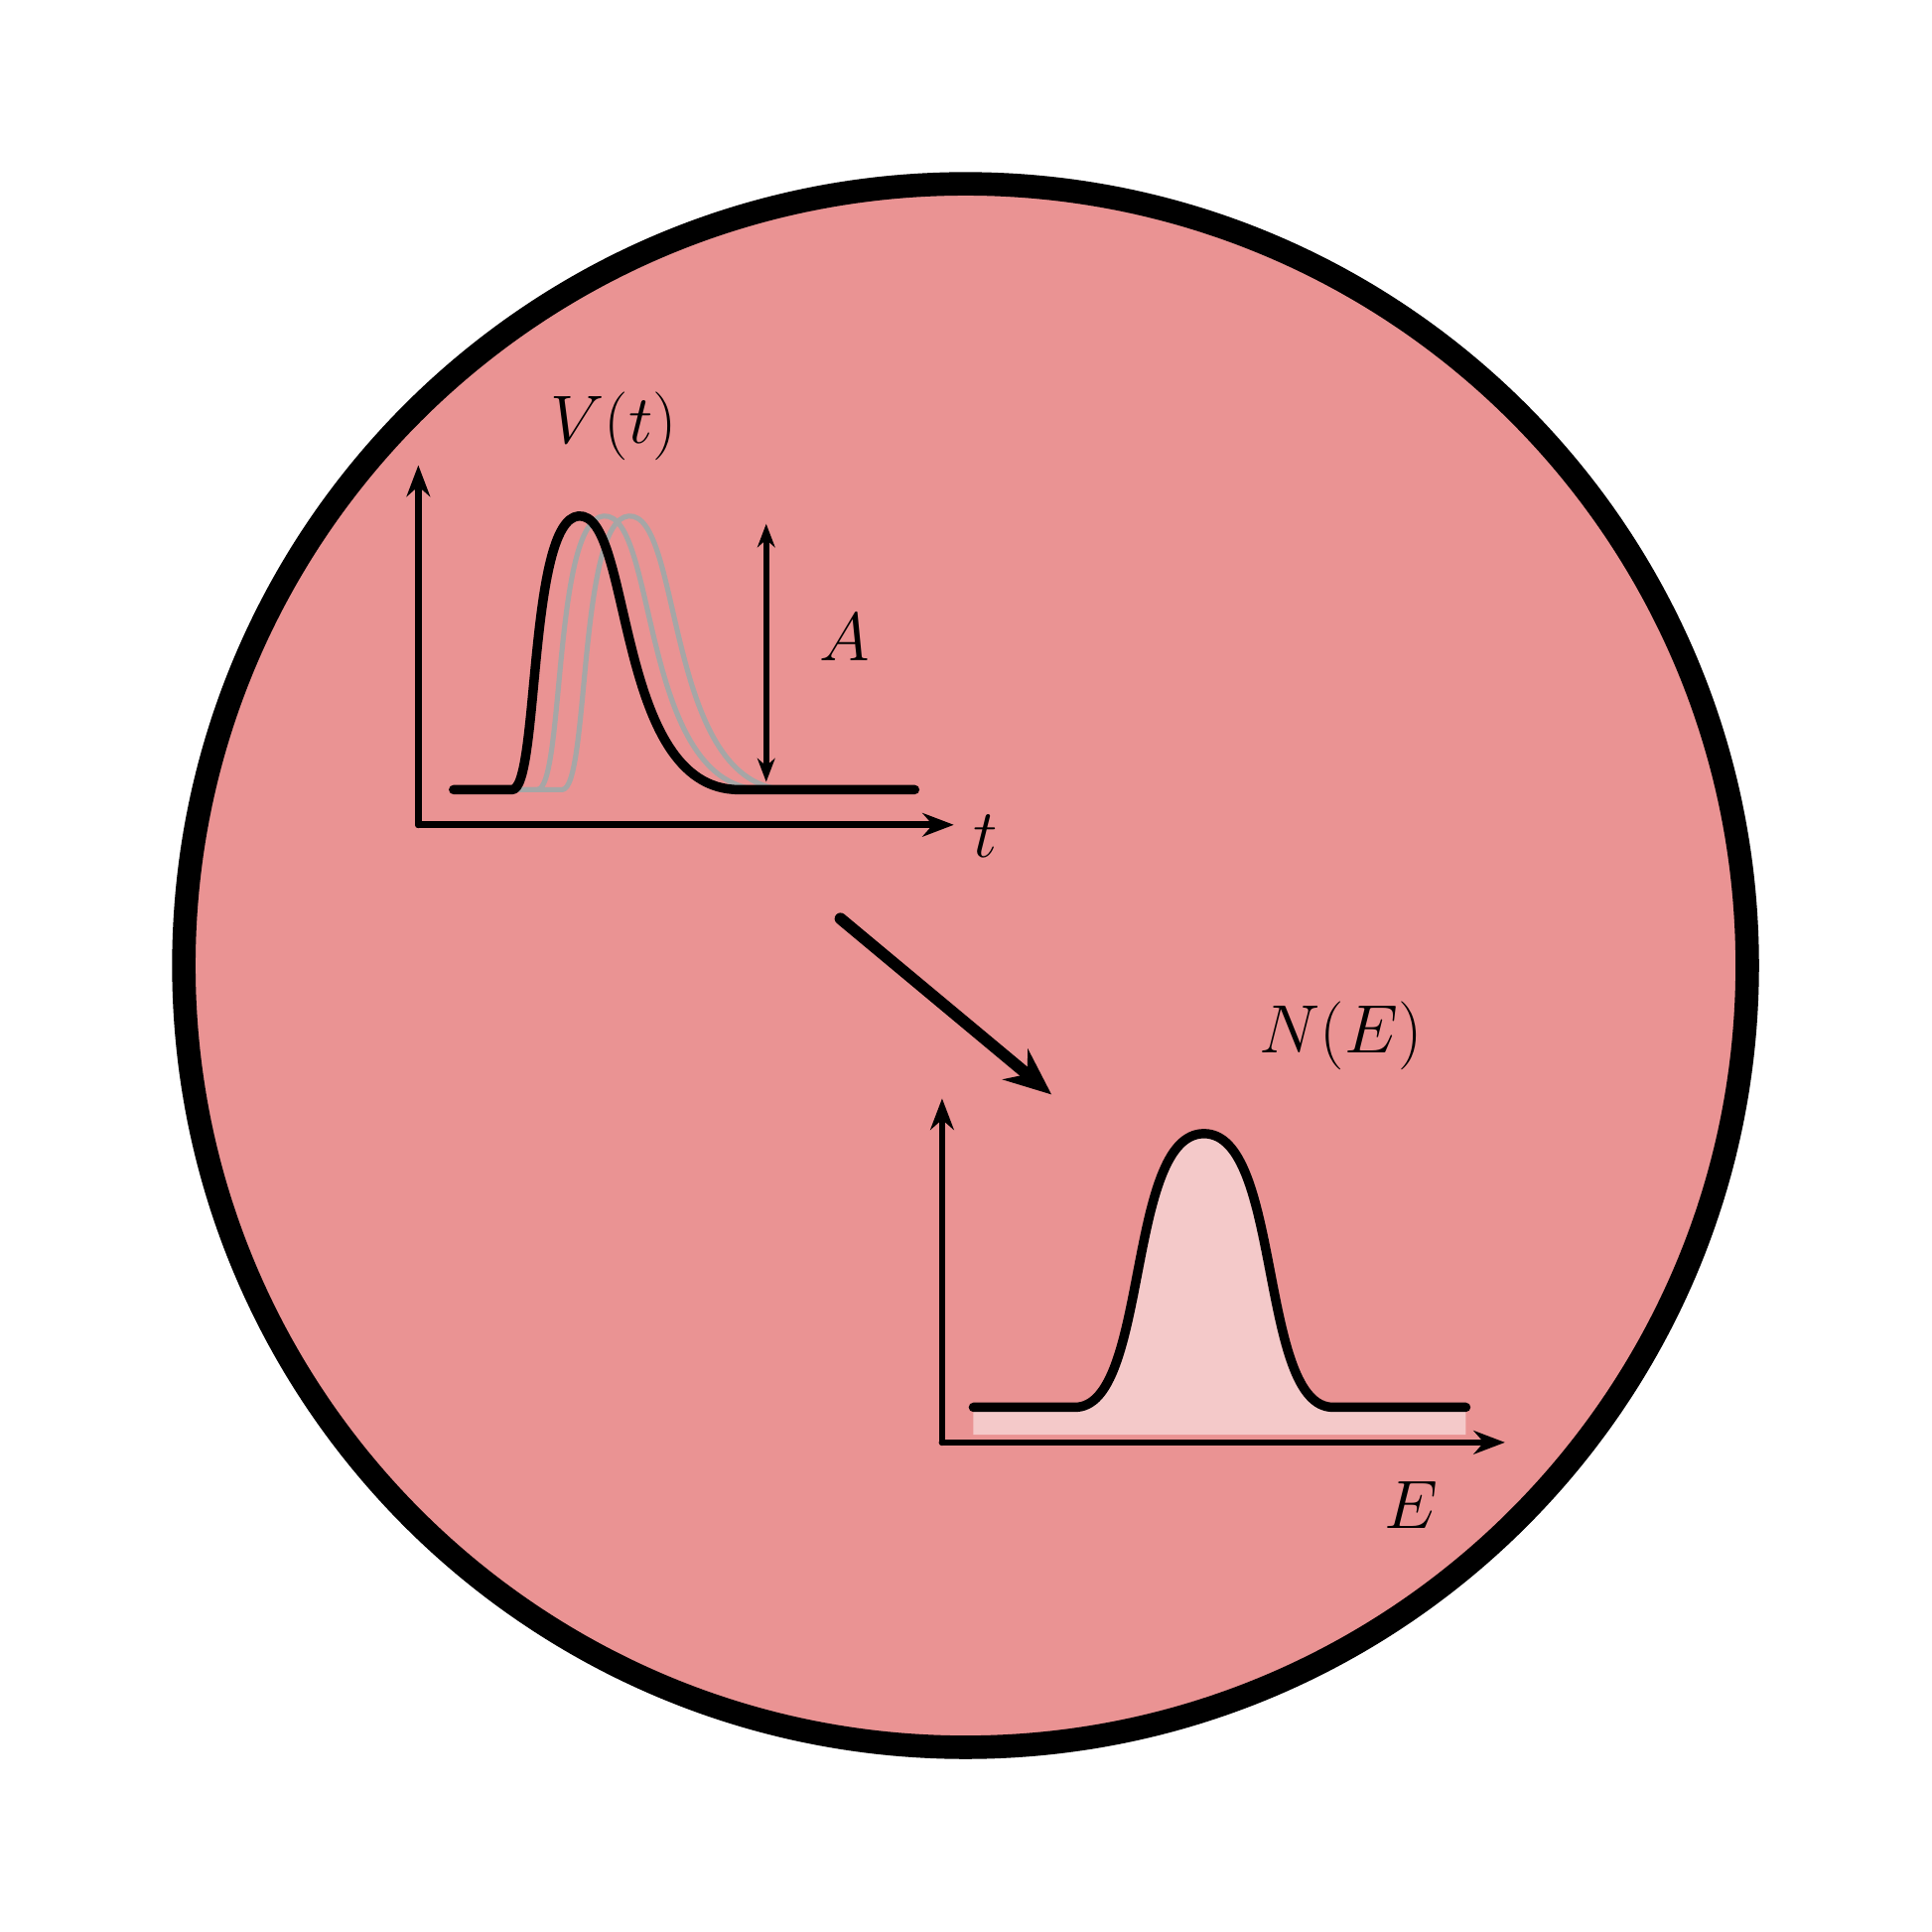
\begin{tikzpicture}[x=10mm,y=10mm,line cap=round,line join=round]
  \path[use as bounding box] (-12,-12) rectangle (12,12);
  \filldraw[fill=badge!50!white,draw=black,line width=3mm] (0,0) circle (10);
  % Illustrative shaped pulses and spectrum; not measured data.
  % The pulse-height estimator is calibrated to energy, then histogrammed
  % over many events. The arrow does not imply a spectrum from one event.
  \begin{scope}
    \draw[black,line width=.85mm,-{Stealth[length=4mm]}] (-7,1.8) -- (-.15,1.8);
    \draw[black,line width=.85mm,-{Stealth[length=4mm]}] (-7,1.8) -- (-7,6.4);
    \node[font=\fontsize{32}{38}\selectfont] at (-4.5,6.9) {$V(t)$};
    \node[font=\fontsize{28}{32}\selectfont] at (.25,1.65) {$t$};
    % Repeated pulses suggest the event ensemble that forms a peak.
    \foreach \shift in {0,.32,.64} {
      \draw[signal!35,line width=.65mm]
        (-6.55,2.25) -- ({-5.8+\shift},2.25)
        .. controls ({-5.45+\shift},2.25) and ({-5.6+\shift},5.7) .. ({-4.95+\shift},5.75)
        .. controls ({-4.25+\shift},5.8) and ({-4.5+\shift},2.25) .. ({-2.9+\shift},2.25)
        -- (-.65,2.25);
    }
    \draw[black,line width=1.2mm]
      (-6.55,2.25) -- (-5.8,2.25)
      .. controls (-5.45,2.25) and (-5.6,5.7) .. (-4.95,5.75)
      .. controls (-4.25,5.8) and (-4.5,2.25) .. (-2.9,2.25) -- (-.65,2.25);
    \draw[accent,line width=.75mm,{Stealth[length=3mm]}-{Stealth[length=3mm]}]
      (-2.55,2.35) -- (-2.55,5.65);
    \node[font=\fontsize{26}{30}\selectfont,text=accent] at (-1.55,4.2) {$A$};
  \end{scope}
  \draw[black,line width=1.5mm,-{Stealth[length=6mm,width=5mm]}] (-1.6,.6) -- (1.1,-1.65);
  \begin{scope}
    \draw[black,line width=.85mm,-{Stealth[length=4mm]}] (-.3,-6.1) -- (6.9,-6.1);
    \draw[black,line width=.85mm,-{Stealth[length=4mm]}] (-.3,-6.1) -- (-.3,-1.7);
    \node[font=\fontsize{30}{36}\selectfont] at (4.8,-.9) {$N(E)$};
    \node[font=\fontsize{28}{32}\selectfont] at (5.7,-6.9) {$E$};
    \path[fill=white,fill opacity=.5]
      (.1,-5.65) -- (1.4,-5.65)
      .. controls (2.35,-5.65) and (2.05,-2.15) .. (3.05,-2.15)
      .. controls (4.05,-2.15) and (3.75,-5.65) .. (4.7,-5.65)
      -- (6.4,-5.65) -- (6.4,-6.0) -- (.1,-6.0) -- cycle;
    \draw[black,line width=1.2mm]
      (.1,-5.65) -- (1.4,-5.65)
      .. controls (2.35,-5.65) and (2.05,-2.15) .. (3.05,-2.15)
      .. controls (4.05,-2.15) and (3.75,-5.65) .. (4.7,-5.65) -- (6.4,-5.65);
  \end{scope}
\end{tikzpicture}
\end{document}
